% !Mode:: "TeX:UTF-8"
%此为章节二模板
%\chapter、\section、\subsection、\subsubsection分别对应一二三四级标题
\chapter{相关理论基础及散热结构设计方案}\label{ch:2}

\section{概述}
本文提出了一种基于嵌入式散热模块的微通道散热技术,该技术通过嵌入嵌入体、微通道散热技术和肋与针鳍结构来增强LTCC基板的传热能力。

\section{流体力学基本原理}

\subsection{流体基本特性}

\noindent 算法示例如下:

\begin{algorithm}[H]
    \KwData{this text}
    \KwResult{how to write algorithm with \LaTeX2e}
    initialization\;
    \While{not at end of this document}{
        read current\;
        \eIf{understand}{
            go to next section\;
            current section becomes this one\;
        }{
            go back to the beginning of current section\;
        }
    }
    \caption{How to wirte an algorithm.}
\end{algorithm}

\subsubsection{流体的压缩性与膨胀性}

\subsubsection{流体的黏性}

\subsection{流体力学控制方程}
在本次研究中应用到计算流体动力学(Computational Fluid Dynamics,CFD)对研究对象进

\subsubsection{连续性方程}
连续性方程表明在连续介质模型的流体域中,流体的质量守恒。
对于不可压缩流体,流体的密度为常数因此其连续性方程为:
\begin{equation}
    \frac{\partial u}{\partial x}+\frac{\partial v}{\partial y}+\frac{\partial v}{\partial z}=0
\end{equation}
u,v,w 分别是 x,y,z 方向的速度分量。

\subsubsection{动量方程}
流体中的动量守恒的物理意义为单位体积流体上所受的力之和等于单位体积流体的动量的时间变化率。
\begin{align}% 式中的&为对齐的位置标记
    u & \frac{\partial u}{\partial x}+v \frac{\partial u}{\partial y}+w \frac{\partial u}{\partial z}=-\frac{1}{\rho_{f}} \frac{\partial p}{\partial x}+\frac{\mu_{f}}{\rho_{f}}\left(\frac{\partial^{2} u}{\partial x^{2}}+\frac{\partial^{2} u}{\partial y^{2}}+\frac{\partial^{2} u}{\partial z^{2}}\right) \\
    u & \frac{\partial v}{\partial x}+v \frac{\partial v}{\partial y}+w \frac{\partial v}{\partial z}=-\frac{1}{\rho_{f}} \frac{\partial p}{\partial y}+\frac{\mu_{f}}{\rho_{f}}\left(\frac{\partial^{2} v}{\partial x^{2}}+\frac{\partial^{2} v}{\partial y^{3}}+\frac{\partial^{2} v}{\partial z^{3}}\right) \\
    u & \frac{\partial w}{\partial x}+v \frac{\partial w}{\partial y}+w \frac{\partial w}{\partial z}=-\frac{1}{\rho_{f}} \frac{\partial p}{\partial z}+\frac{\mu_{f}}{\rho_{f}}\left(\frac{\partial^{2} w}{\partial x^{2}}+\frac{\partial^{2} w}{\partial y^{2}}+\frac{\partial^{2} w}{\partial z^{2}}\right)
\end{align}
$\rho_{f}$ 和 $\mu_{f}$ 分别是冷却剂的密度和动态粘度,p 是冷却剂压力。

\subsubsection{能量方程}
能量方程即为能量守恒定律在流体上的数学描述,表示流体在流动过程中单位体积流体的总能量等于其增加的热量与单位时间内体积力和表面力所做的功之和。
\begin{equation}
    u \frac{\partial T_{f}}{\partial x}+v \frac{\partial T_{f}}{\partial y}+w \frac{\partial T_{f}}{\partial z}=\frac{k_{f}}{\rho_{f} C_{ f}}\left(\frac{\partial^{2} T_{f}}{\partial x^{2}}+\frac{\partial^{2} T_{f}}{\partial y^{2}}+\frac{\partial^{2} T_{f}}{\partial z^{2}}\right)
\end{equation}
其中,$C_{f}$ 为冷却剂的比热容,$T_{f}$ 为液体的温度,$k_{f}$ 为流体的热导率。

\begin{equation}
    k_{s}\left(\frac{\partial^{2} T_{s}}{\partial x^{2}}+\frac{\partial^{2} T_{s}}{\partial y^{2}}+\frac{\partial^{2} T_{s}}{\partial z^{2}}\right)=0
\end{equation}
其中$T_{s}$为固体温度,$k_{s}$为固体导热率。

接下来是内容……

\subsection{结构设计思路}

\begin{enumerate}
    \item 在基板内部进行微通道散热以缩短传热路径,见\cref{fig:LTCC-Microchannels};
    \item 在基板内嵌入散热模块减少整体热阻,提高热传导效率,见\cref{fig:Embedded-cooling-module};
    \item 在嵌入式散热模块上制作针鳍或肋增强对流传热,以进一步减小热阻,见\cref{fig:Rib-pin-fin}。
\end{enumerate}

\begin{figure}[htb]
    \subfloat[改进前的结构]{
        \label{fig:Unimproved-cooling-structure}
        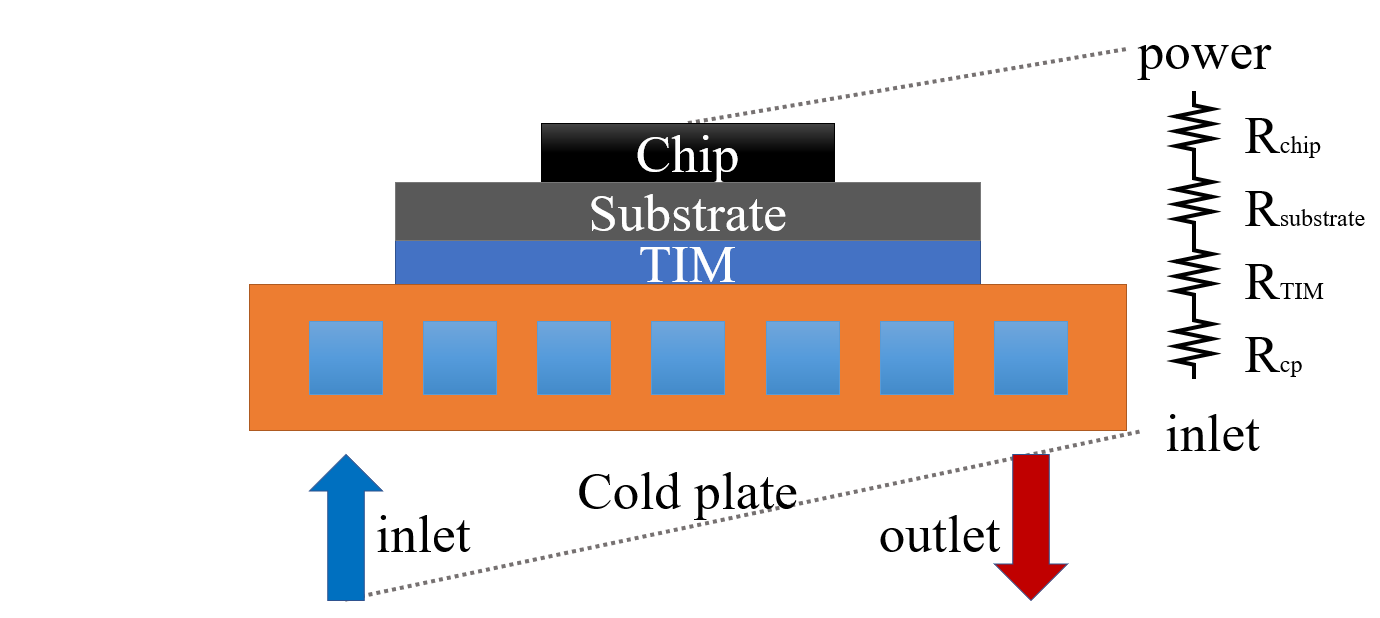
\includegraphics[width=0.45\linewidth]{Unimproved-cooling-structure.png}}
    \subfloat[基板内进行微通道散热]{
        \label{fig:LTCC-Microchannels}
        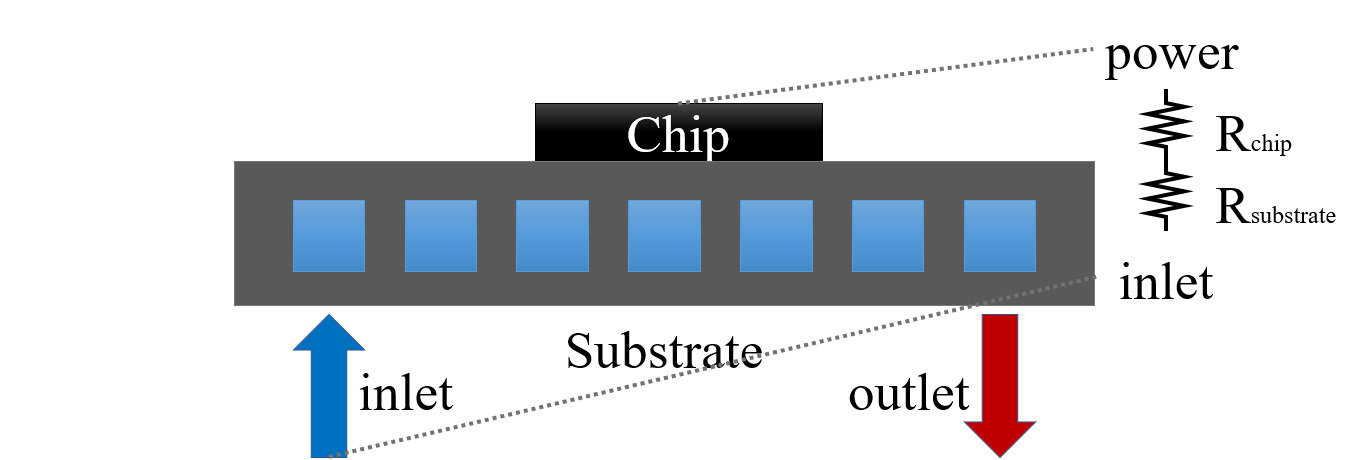
\includegraphics[width=0.45\linewidth]{LTCC-Microchannels.png}}

    \subfloat[嵌入散热模块]{
        \label{fig:Embedded-cooling-module}
        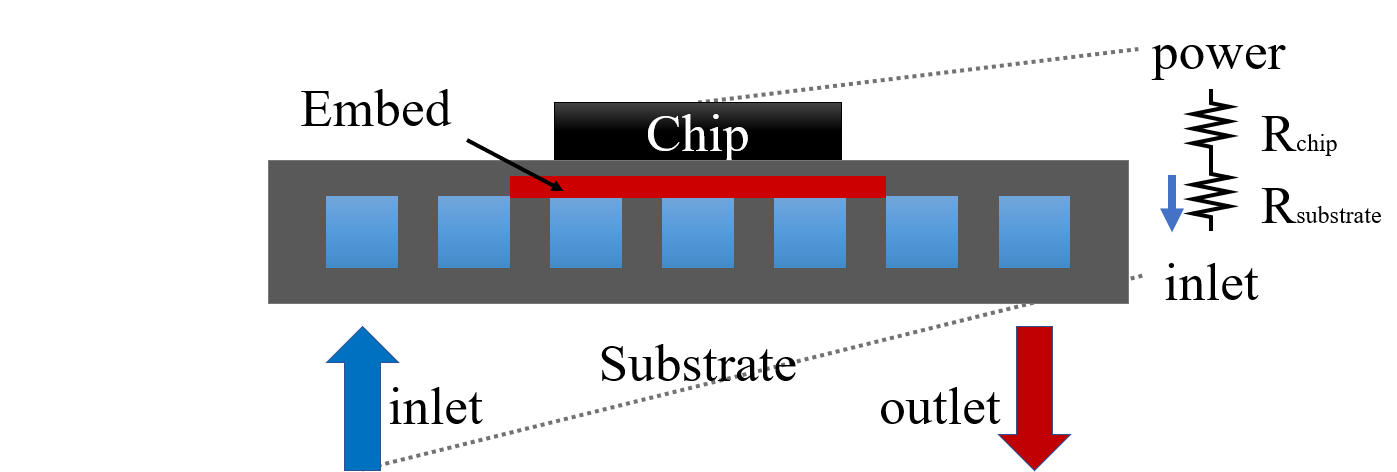
\includegraphics[width=0.45\linewidth]{Embedded-cooling-module.png}}
    \subfloat[带针鳍或肋的嵌入式散热模块]{
        \label{fig:Rib-pin-fin}
        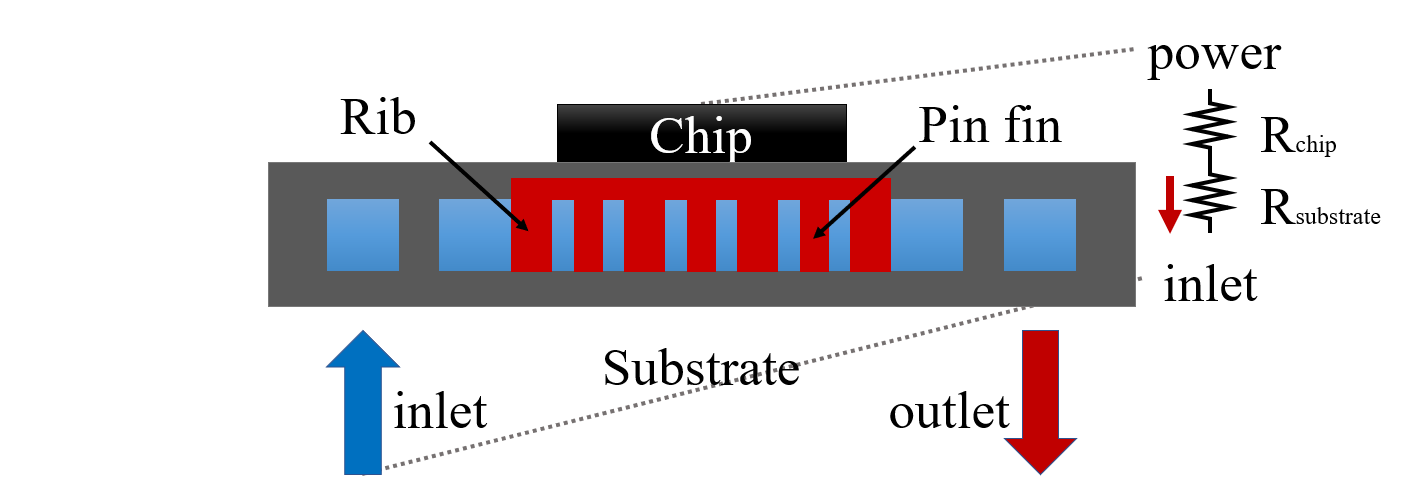
\includegraphics[width=0.45\linewidth]{Rib-pin-fin.png}}
    \caption{三种强化传热途径示意图}
    \label{fig:Three-enhanced-heat-transfer-paths}
\end{figure}

\section{本章小节}
本章介绍了基于嵌入式散热模块的微通道散热技术所涉及的基……